% !Mode:: "TeX:UTF-8"

\titlepage

% \begin{frame}{说在前面}
% 	\linespread{1.5}
% 	  \begin{itemize}[<+-|alert@+>]
% 	    \item \ba{雷同!!!}
% 	    \item 本子太烂了就换本新的吧
% 	    \item 本子还不算特别烂的下学期请继续使用
% 	    \item 新本子:贴照片,写上姓名、专业、学号、籍贯
% 	  \end{itemize}
% \end{frame}

% \begin{frame}{需要注意的问题}
% 	\linespread{1.5}
% 	  \begin{itemize}%[<+-|alert@+>]
% 	    \item L'Hospital法则
% 	    \begin{itemize}
% 	      \item \it 只能应用于“$\df{\bm{0}}{\bm{0}}$”
% 	      和“$\df{\bm{\infty}}{\bm{\infty}}$”型
% 	      \item \it 及时使用无穷小代换进行简化
% 	      \item \it 不正规的符号:\b 
% 	      $\xlongequal{\footnotesize\mbox{“L”}}$、
% 	      $\xlongrightarrow{\footnotesize\mbox{“L'Hospital法则”}}$、
% 	      $\df{\bm{0}}{\bm{0}}$、$\df{\bm{\infty}}{\bm{\infty}}$
% 	    \end{itemize}
% 	    \item Taylor公式
% 	    \begin{itemize}
% 	      \item \it Taylor多项式不包含余项
% 	      \item \it 合并同次幂的系数
% 	      \item \it 尽量按照幂次由低到高排列,最后写余项
% 	    \end{itemize}
% 	  \end{itemize}
% \end{frame}

% \section{12.3 幂级数及其应用}

\begin{frame}
	\linespread{1.5}
	\ba{1.求下列函数项级数的收敛域:
	
	\bs
	
	(1)$\df x{1\cdot 3}+\df{x^2}{2\cdot3^2}++\df{x^3}{3\cdot3^3}
	+\ldots++\df{x^n}{n\cdot3^n}+\ldots$}
	
	\bigskip
	
	\small 解:\it
	因为
	$$\limn\sqrt[n]{\df1{n\cdot 3^n}}=\df13,$$
	故该级数的收敛区间为$(-3,3)$。
	
	又$x=3$时,级数为$\sumn\df1n$,发散;
	$x=-3$时,级数为$\sumn\df{(-1)^n}n$,收敛。
	故所求收敛域为$[-3,3)$。
\end{frame}

\begin{frame}
	\linespread{1.5}
	\ba{(2)$\sumn\df{(2x+1)^n}n$}
	
% 	\bigskip
	
	\small 解:\it
	令$y=2x+1$,考虑级数$\sumn\df{y^n}n$。因为$\limn\sqrt[n]{\df1n}=1$,
	故其收敛区间为$(-1,1)$。
	
	又$y=1$时,级数为$\sumn\df1n$,发散;
	$y=-1$时,级数为$\sumn\df{(-1)^n}n$,收敛。故级数$\sumn\df{y^n}n$
	的收敛域为$y\in[-1,1)$。相应地,原级数的收敛域为$x\in[-1,0)$。
\end{frame}

\begin{frame}
	\linespread{1.5}
	\ba{(3)$\sumn(-1)^n\df{x^{2n+1}}{2n}$}
	
% 	\bigskip
	
	\small 解:\it
	$\sumn(-1)^n\df{x^{2n+1}}{2n}=x\cdot\sumn(-1)^n\df{x^{2n}}{2n}$,
	由此可知原级数与级数$\sumn(-1)^n\df{x^{2n}}{2n}$同敛散。
	
	令$y=x^2$,考虑级数$\sumn(-1)^n\df{y^{n}}{2n}$。因为
	$\limn\sqrt[n]{\df1{2n}}=1$,故该级数的收敛区间为$(-1,1)$。
	相应地,级数$\sumn(-1)^n\df{x^{2n}}{2n}$与原级数的收敛区间均为$(-1,1)$。
	
	又$x=\pm1$时,原级数为$\sumn\df{(-1)^n}{2n}$,由Leibniz判别法,收敛。
	故原级数的收敛域为$[-1,1]$。
\end{frame}

\begin{frame}
	\linespread{1.5}
	\ba{(4)$\sumn\sin\df 1 {3n}\left(\df{3+x}{3-2x}\right)^n$}
	
% 	\bigskip
	
	\small 解:\it
	令$y=\df{3+x}{3-2x}$,考虑级数$\sumn y^n\sin\df1{3n}$。
	因为
	$$\limn\df{\sin\frac1{3n}}{\sin\frac1{3(n+1)}}=1,$$
	故该级数的收敛区间是$(-1,1)$。
	
	又$y=1$时,级数为$\sumn\sin\df1{3n}$,因为$\limn n\sin\df1{3n}=\df13$,
	故由比较判别法,级数发散;$y=-1$时,级数为$\sumn(-1)^n\sin\df1{3n}$,
	由Leibniz判别法,收敛。故级数$\sumn y^n\sin\df1{3n}$的收敛域为
	$[-1,1)$。求解不等式$-1\leq\df{3+x}{3-2x}<1$,
	可得$x\in(-\infty,0)\cup[6,+\infty)$,即为所求原级数的收敛域。\fin
\end{frame}

\begin{frame}
	\linespread{1.5}
	\ba{2.求下列级数的和函数:
	(1)$\sumn(-1)^{n-1}nx^{n-1}$}
	
% 	\bigskip
	
	\small 解:\it
	令$y=-x$,考虑级数$\sumn ny^{n-1}$,易得该级数的收敛域为$(-1,1)$。
	设其和函数为$S(y)$,于是当$y\in(-1,1)$时,
	$$\dint_0^yS(t)\d t=\dint_0^y\sumn nt^{n-1}\d t
	=\sumn \dint_0^ynt^{n-1}\d t=\sumn y^n=\df1{1-y}-1,$$
	进而可得
	$$S(y)=\df1{(1-y)^2}.$$
	综上,
	$$\sumn(-1)^{n-1}nx^{n-1}=\df1{(1+x)^2},\quad x\in(-1,1).$$
\end{frame}

\begin{frame}
	\linespread{1.5}
	\ba{(2)$\df1a+\df{2x}{a^2}+\ldots+\df{nx^{n-1}}{a^n}+\ldots$,其中$a>0$.}
	
	\bigskip
	
	\small 解:\it
	该级数即为$\df1a\sumn n\left(\df xa\right)^{n-1}$,易得其收敛域为$(-a,a)$。
	记$y=\df xa$,由$(1)$的结果可得
	\begin{align*}
		\df1a\sumn n\left(\df xa\right)^{n-1}
		&=\df1a\sumn ny^{n-1}=\df1a\df1{(1-y)^2}\\
		&=\df1a\df1{\left(1-\frac
		xa\right)^2} =\df{a}{(a-x)^2}.
	\end{align*}
	即为所求。
\end{frame}

\begin{frame}
	\linespread{1.5}
	\ba{(3)$\sumn[0]\df{x^{2n+1}}{n!}$}
	
	\bigskip
	
	\small 解:\it
	该级数的收敛域为$(-\infty,+\infty)$。令$y=x^2$
	$$\sumn[0]\df{x^{2n+1}}{n!}=x\sumn[0]\df{x^{2n}}{n!}
	=x\sumn[0]\df{y^n}{n!}.$$
	级数$\sumn[0]\df{y^n}{n!}$当$y\in(-\infty,+\infty)$时收敛于$e^y$。
	由此即知
	$$\sumn[0]\df{x^{2n+1}}{n!}=xe^{x^2},\quad x\in(-\infty,+\infty).$$
	\fin
\end{frame}

\begin{frame}
	\linespread{1.5}
	\ba{3.将下列函数展开成Maclaurin级数,并求其收敛域:
	
	(1)$f(x)=\df1{x^2-4x+3}$}
	
	\bigskip
	
	\small 解:\it
	\begin{align*}
		\df1{x^2-4x+3}&=\df12\left(\df1{1-x}-\df13\df1{1-\frac x3}\right)\\
		&=\df12\left(\sumn[0]x^n-\df13\sumn[0]\df{x^n}{3^n}\right)\\
		&=\df12\sumn[0]\left(1-\df1{3^{n+1}}\right)x^n.
	\end{align*}
	该级数的收敛域为$[-1,1)$。
\end{frame}

\begin{frame}
	\linespread{1.5}
	\ba{(2)$f(x)=\df 1{1+x+x^2}$}
	
	\bigskip
	
	\small 解:\it
	\begin{align*}
		\df 1{1+x+x^2}
		&=\df{1-x}{1-x^3}=(1-x)\sumn[0]x^{3n}\\
		&=1-x+x^3-x^4+x^6-x^7+\ldots+x^{3n}-x^{3n+1}+\ldots.
	\end{align*}
	注意到级数$\sumn[0]x^{3n}$的收敛域为$(-1,1)$,故以上级数的收敛域为$(-1,1)$。\fin
\end{frame}

\begin{frame}
	\linespread{1.5}
	\ba{4.将函数$f(x)=\df1{\sqrt{3+2x-x^2}}$展开成$x=1$处的幂级数,并求其收敛区间。}
	
	\bigskip
	
	\small 解:\it
	\begin{align*}
		f(x)
		&=\df12\left[1-\left(\df{x-1}2\right)^2\right]^{-\frac12}
		=\df12\sumn[0]{\left(\begin{array}{c}
			-\frac12 \\ n
		\end{array}\right)}\left[-\left(\df{x-1}2\right)^2\right]^n\\
		&=\sumn[0]\df{(2n-1)!!}{2^{2n+1}(2n)!!}(x-1)^{2n}
	\end{align*}
	注意到
	$$\limn\df{\frac{(2n+1)!!}{2^{2n+3}(2n+2)!!}}{\frac{(2n-1)!!}{2^{2n+1}(2n)!!}}=\df12,$$
	故所得级数的收敛半径为$2$,相应地收敛区间为$(-1,3)$。
	\fin
\end{frame}

\begin{frame}
	\linespread{1.5}
	\ba{5.已知$f_n(x)\;(n\in\mathbb{Z}^+)$满足
	$$f'_n(x)=f_n(x)+x^{n-1}e^x,$$
	且$f_n(1)=\df en$,求级数$\sumn f_n(x)$的和。}
	
	\bigskip
	
	\small 解:\it
	由已知等式,可得
	$$\left[f_n(x)e^{-x}\right]'=x^{n-1},$$
	进而可知
	$$f_n(x)=\left(\df{x^n}n+C\right)e^x.$$
	注意到$f_n(1)=\df en$,可得$C=0$,故$f_n(x)=\df{x^n}ne^x$。
\end{frame}

\begin{frame}
	\linespread{1.5}
	\small\it
	
	$$\sumn f_n(x)=\sumn\df{x^n}ne^x=e^x\sumn\df{x^n}n.$$
	
	考虑级数$\sumn\df{x^n}n$,易得其收敛域为$[-1,1)$。设其和函数为$S(x)$,则
	$$S'(x)=\left[\sumn\df{x^n}n\right]'
	=\sumn\left[\df{x^n}n\right]'=\sumn x^{n-1}=\df1{1-x}.$$
	从而
	$$S(x)=\dint_0^x\df1{1-t}\d t=-\ln|1-x|,\quad x\in[-1,1),$$
	进而
	$$\sumn f_n(x)=-\df{e^x}\ln|1-x|,\quad x\in[-1,1).$$
	\fin
\end{frame}

\begin{frame}{出现的问题}
	\linespread{1.5}
	  \begin{itemize}%[<+-|alert@+>]
	    \item 作业进度慢!
	    \item 概念问题
	    \begin{itemize}
	      \item \b\it 幂级数展开不熟练
	      \item \b\it Maclaurin级数和关于$(x-x_0)$的幂级数分不清
	    \end{itemize}
	    \item 过程不规范或不完整
	    \begin{itemize}
	      \item \b\it 求收敛域要单独讨论端点的敛散性
	      \item \b\it 相同幂次的项要合并,并按幂次从小到大排列
	      \item \b\it 书写潦草随意\pause
	    \end{itemize}
	    \item \ba{雷同!!!}
	  \end{itemize}
\end{frame}

% \begin{frame}
% 	\linespread{1.5}
% 	\ba{3.设$D$是由曲线$y=\sin x+1$与三条直线$x=0,x=\pi,y=0$
% 	所围成的曲边梯形,求$D$绕$x$轴旋转一周所围成的旋转体的体积。
% 	}
% 	\pause
% 	
% % 	\bigskip
% 	
% 	\begin{columns}
% 		\begin{column}{.5\textwidth}
% 			\begin{center}
% 				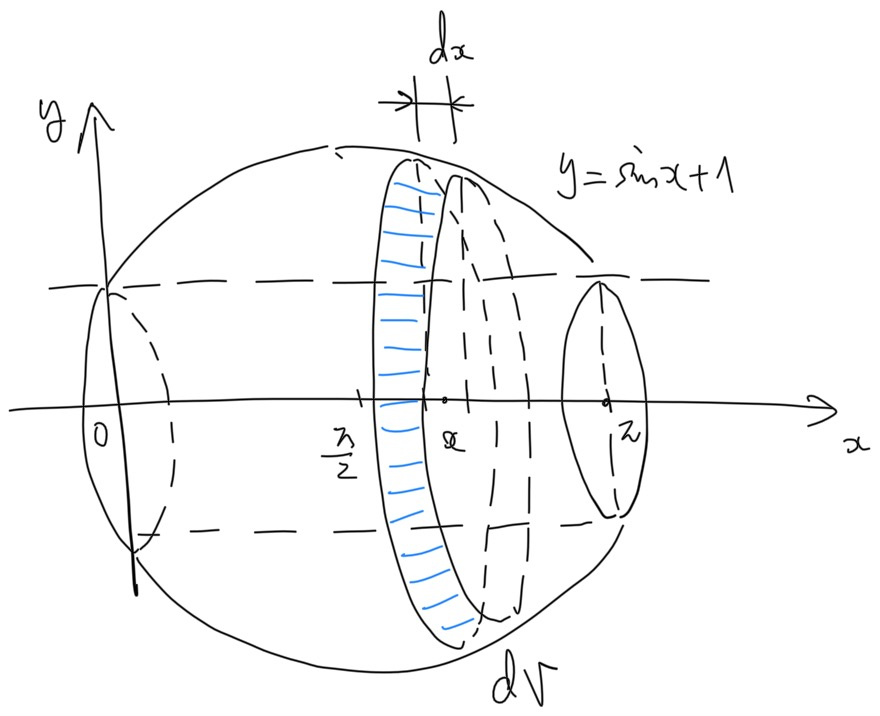
\includegraphics[width=.9\textwidth]{./images/ch6/sinx1cs.jpg}
% 		% 		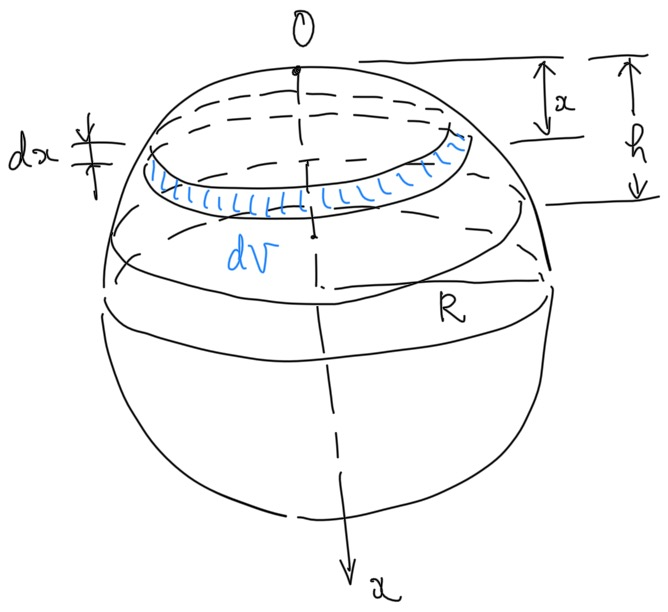
\includegraphics[width=6cm]{./images/ch6/topSp.jpg}
% 			\end{center}		
% 		\end{column}
% 		\begin{column}{.5\textwidth}
% 			\small 解:\it
% 			如图,体积微元$\d V=\pi y^2\d x$,	故所求体积
% 			$$
% 				V=\dint_0^{\pi}\pi(\sin x+1)^2\d x=\df32\pi^2.
% 			$$
% 		\end{column}
% 	\end{columns}
% \end{frame}